  \section{Ejercicio 7}

\subsection{Introducción}
En este ejercicio se busca comparar las diferentes heurísticas y metaheuríticas halladas para resolver el problema de encontrar el máximo subgrafo común entre dos grafos. Para ello no sólo se compararán los tiempos de ejecución sino que también se tomará en cuenta cuántas aristas tiene el grafo solución para cada uno de los algoritmos. Este resultado se lo comparará, en los casos en los que sea posible, con los resultados obtenidos en el algoritmo exacto, es decir, se observará qué tan lejos de la solución óptima se encuentra el resultado obtenido con los algoritmos heurísticos. Esto no es posible de hacer en cualquier caso ya que, como sabemos, el algoritmo exacto resuelve un problema de tipo NP-completo y si se corre el algoritmo con un grafo de tamaño muy grande tardaría muchísimo tiempo en devolver un resultado. Para poder comparar con el resultado correcto se utilizarán grafos especiales ($C_n$, bipartito, bipartito completo, $K_n$, árboles (que son una clase particular de bipartitos), estrellas (también bipartitos, son $K_{1n}$), cografos, etc) ya que al utilizarlos se puede calcular de forma manual cuántas aristas en común tienen los grafos o se puede correr el algoritmo y que sea exacto sin que tarde demasiado tiempo (como es el caso de los cografos y completos).

\subsection{Experimentación}
    
\subsubsection*{Experimento 1}\;
 El objetivo de este experimento fue extraer conclusiones acerca de la variación en el tiempo de cómputo requerido por cada una de las heurísticas cuando se varían los valores de $n_1$ dejando $m_1$ $=$ 3$n_1$. \\
 Esperaremos que el experimento determine que la heurística mas rápida es la golosa, seguida de de búsqueda local y por ultimo la Tabú, nuestro fundamento para esto esta en que cada una es una ampliación de la anterior, es decir la búsqueda local, primero usa la heurística golosa y la Tabú usa reiteradamente el proceso(muy similar a) búsqueda Local.\\

Para ello se utilizará un generador de grafos que funciona de la siguiente manera: dada una cantidad de nodos y aristas, en cada paso crea una nueva arista con extremos válidos (es decir, entre 0 y la cantidad de nodos - 1) y que no esté repetida (que no haya sido creada todavía).\\
Para las heurísticas que cuentan con más de una versión (aquellas que tienen diferentes criterios para determinar lo que es una vecindad, o como la heurística de búsqueda tabú que se puede variar el tamaño de la misma, los vecinos a tener en cuenta en cada iteración y el criterio de parada) se tomó la combinación de variantes que dio mejores resultados en los experimentos realizados para el análisis particular de cada una de ellas.\\
Se sabe que para comparar bien las heurísticas es necesario variar todas las combinaciones de parámetros pero a fines de este TP, y para mantener acotado el alcance del mismo, dada la cantidad de experimentos que hemos hecho, vamos a experimentar con grafos con la misma cantidad de vértices y de aristas.

\subsubsection*{Datos de entrada}\;
\noindent Los valores de $n_1$ tomados fueron desde $10$ hasta $70$ de $5$ en $5$. \\
       Los valores de $n_2$ y $m_2$ fueron $50$ y $500$ respectivamente. Los valores de $tamanoMaximoListaTabu$ y $k$ fue $10$. El valor de $cuantosVecinosMiro$, tanto para la heurística de búsqueda local como para tabú, fue $20$. Estos valores fueron elegidos de forma arbitraria. \\
        Para generar los grafos de forma aleatoria se utilizó el generador-grafo-rapido.cpp que se encuentra en la carpeta src y para correrlo se utilizó el exp1.sh que se encuentra en la carpeta exp/ejercicio7/exp1. \\
        Con el fin de acercarse a los valores reales y descartar posibles falsos resultados, se ejecuta la resolución del problema para cada una de los valores de $n_1$ cinco veces considerando luego el promedio entre los valores obtenidos pero graficando también el desvío estándar (la cantidad de repeticiones a realizar fue elegida arbitrariamente).\; 

\subsubsection*{Resultados}\;
    \begin{figure}[H]
      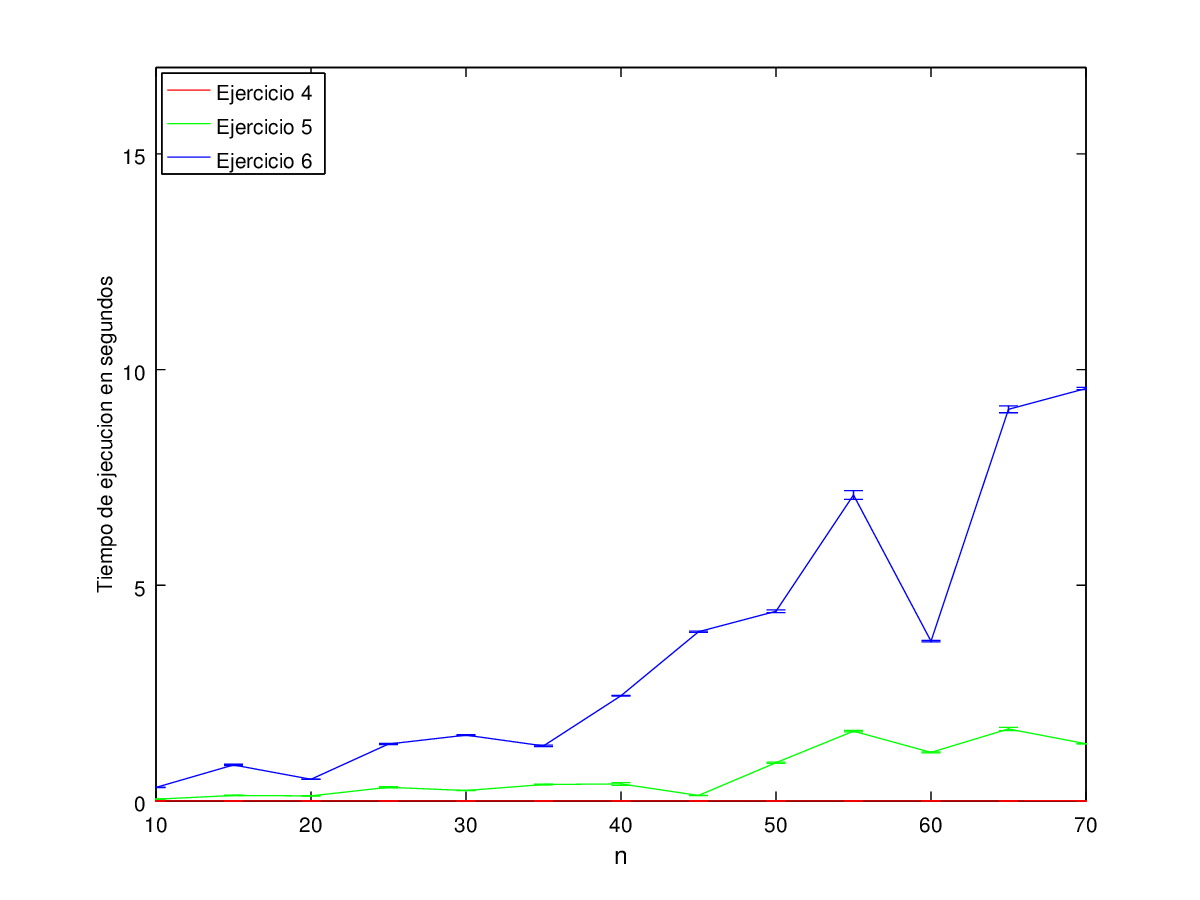
\includegraphics[height=10cm]{graficos/ejercicio7-exp1-tiempos.png}
       \caption{Experimento 1 - Comparando tiempos}
	\end{figure}

\subsubsection*{Conclusiones}\;
Como era esperado, El experimento muestra en el gráfico, como el en cuanto a tiempos de computo, lo mas rápido el la heurística golosa, en segundo lugar la búsqueda local y por ultimo la meta-heurística Tabú.Esto era de esperarse dado que cada una esta comprendida dentro de la anterior como ya explicamos. Por lo que es esperable que los tiempos de computo vayan en incremento, a su vez también sera esperable que la calidad de las soluciones también sea en aumento, ya que si una solución la encontró la heurística golosa, seguro también la encontró la local y también seguro la búsqueda Tabú.\\
Por ultimo notamos la magnitud de la diferencia en el tiempo tardado, la diferencia entre la golosa y la local, es significativa pero tal vez mas aceptable que la Tabu, que su tiempo tiene picos mucho mas altos.\\
Esto nos hace concluir que incluso que la tabú resulte mejor en calidad de solución, puede que para ciertos problemas en donde la performance sea un factor decisivo se prefiera usar la heurística de búsqueda local e incluso la golosa.

\subsubsection*{Experimento 2}\;
 El objetivo de este experimento fue extraer conclusiones acerca de la variación en la cantidad de aristas que contiene el subgrafo respuesta para cada una de las heurísticas cuando se varían los valores de $m$ y $n$ modificando los dos grafos al mismo tiempo pero siempre manteniendo $n_1$ igual a $n_2$ y $m_1$ igual a $m_2$. \\
Para ello, para cada cantidad de nodos se definirá una función para determinar la cantidad de aristas que tendrá el grafo. Estas funciones son las mismas que en el experimento anterior.\\
Al igual que antes, para las heurísticas que cuentan con mas de una versión, se tomó la combinación de variantes que dió mejores resultados en los experimentos realizados para el análisis particular de cada una de ellas.\\
Para generar los grafos con estas cantidades de aristas y nodos se utilizó el mismo generador que en el experimento anterior.\\

\subsubsection*{Datos de entrada}\;

Este experimento tiene los mismos datos de entrada que el anterior y se genera de la misma manera. Al generar uno automáticamente se crea el otro.

\subsubsection*{Resultados}\;
  \begin{figure}[H]
      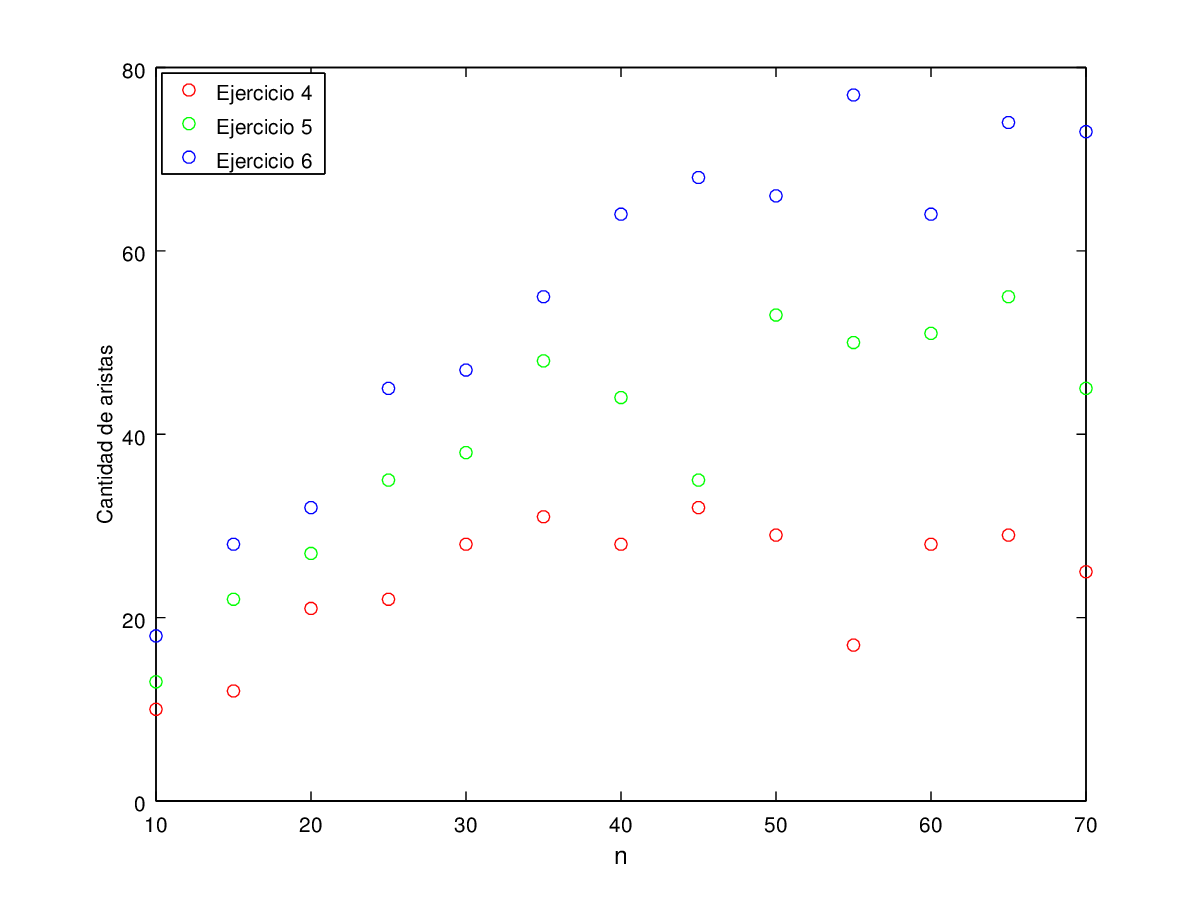
\includegraphics[height=10cm]{graficos/ejercicio7-exp2-aristas.png}
       \caption{Experimento 2 - Comparando aristas}
	\end{figure}
    
\subsubsection*{Conclusiones}\;

Como se puede observar, las heurísticas que requieren mayor tiempo de ejecución son las que dan mejores resultados por lo que no se puede comparar de manera directa entre todas las heurísticas(no se puede determinar una que sea absolutamente mejor). Dependiendo de cuál es la característica que se desea priorizar se elegirá una heurística. Por ejemplo, supongamos el caso de una empresa encargada de repartir correo a la que le llegan las cartas con las direcciones a donde deben ser enviadas muy poco tiempo antes de que los carteros deban salir a repartirlas. Sea el algoritmo que determina cual es el camino mas eficiente para recorrer las calles de la ciudad de tipo NP-completo para el que se desarrollan heurísticas para aproximar en menor tiempo el camino buscado. En este caso convendrá utilizar las heurísticas que requieran poco tiempo de ejecución sin importar si la solución no fue la mejor que se pudo obtener ya que los carteros deben salir a horario. \\
En cambio, el caso de una empresa que necesita cada 5 años éste cálculo convendrá utilizar la heurística más exacta posible ya que no importa mucho cuánto tiempo tarde en ejecutarse.\\ 
Para poder analizar un caso genérico debemos dejar constante una de las dos variables que tenemos (tiempo y correctitud). Como no se tiene control sobre la solución que brinda cada heurística lo que se puede hacer es dejar el tiempo fijo y hacer que todas terminen una vez pasado ese tiempo. Luego se comparará cuál es el resultado que cada algoritmo calculó hasta el momento y ahí sí podemos decir que para cierta instancia una se comporta mejor que la otra.

\subsubsection*{Experimento 3}\;
En este experimento compararemos los resultados que se obtienen de cada heurística cuando se ejecutan todas una misma cantidad de tiempo.\\
Para ello, para cada cantidad de nodos se definirá una función para determinar la cantidad de aristas.\\
Al igual que antes para las heurísticas que cuentan con más de una versión se tomó la combinación de variantes que dio mejores resultados en los experimentos realizados para el análisis particular de cada una de ellas.\\


\subsubsection*{Datos de entrada}\;
\noindent Los valores de $n_1$ tomados fueron desde $10$ hasta $70$ de $5$ en $5$. \\
       Los valores de $n_2$ y $m_2$ fueron $50$ y $200$ respectivamente. Los valores de $tamanoMaximoListaTabu$ y $k$ fue $10$. El valor de $cuantosVecinosMiro$, tanto para la heurística de búsqueda local como para tabú, fue $20$. Estos valores fueron elegidos de forma arbitraria. \\
        Para generar los grafos de forma aleatoria se utilizó el generador-grafo-rapido.cpp que se encuentra en la carpeta src y para correrlo se utilizó el exp3.sh que se encuentra en la carpeta exp/ejercicio7/exp3. \\
        Con el fin de acercarse a los valores reales y descartar posibles falsos resultados, se ejecuta la resolución del problema para cada una de los valores de $n_1$ cinco veces considerando luego el promedio entre los valores obtenidos pero graficando también el desvío estándar (la cantidad de repeticiones a realizar fue elegida arbitrariamente).\; 
\subsubsection*{Resultados}\;
  \begin{figure}[H]
      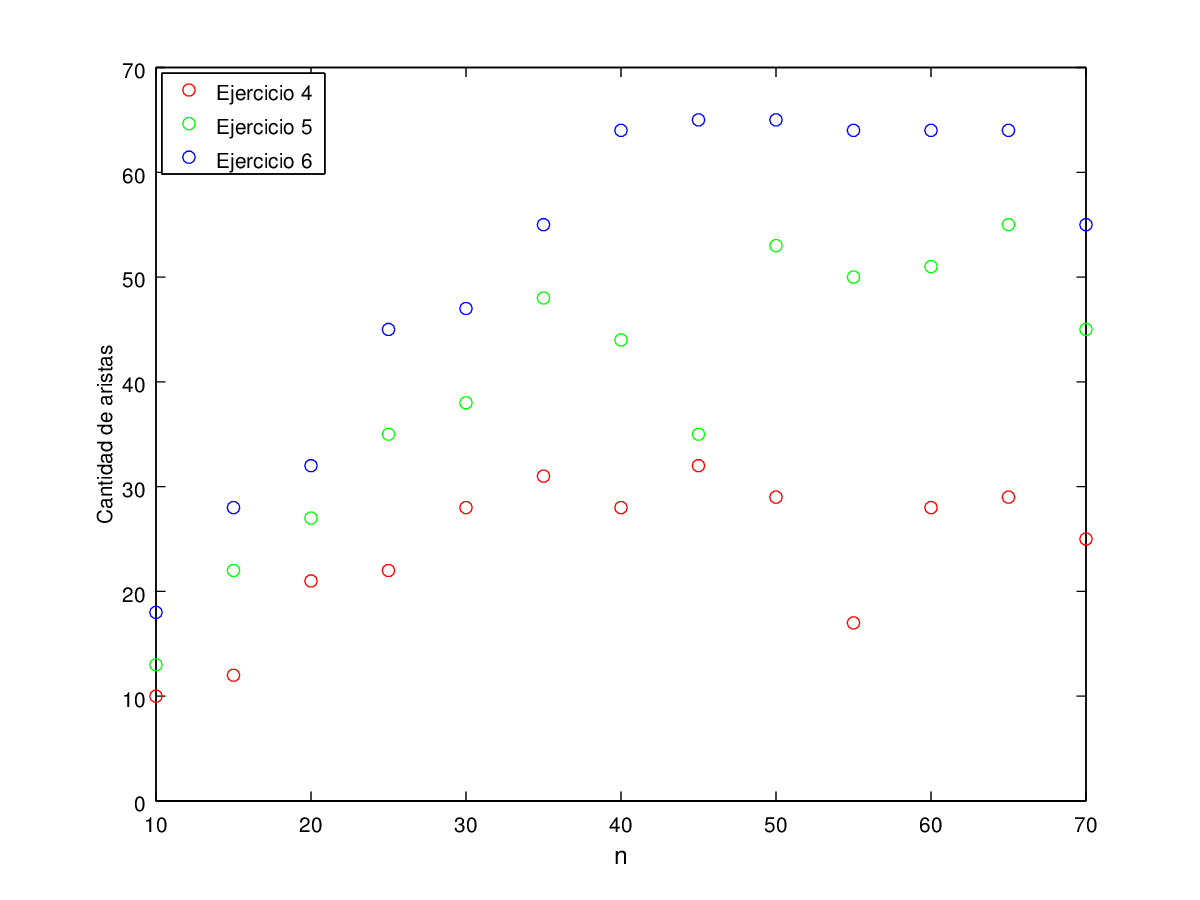
\includegraphics[height=10cm]{graficos/ejercicio7-exp3-aristas.png}
       \caption{Experimento 3}
	\end{figure}
    
    
\subsubsection*{Conclusiones}\;


Hasta ahora ya realizamos las comparaciones entre las heurísticas desarrolladas a lo largo de este trabajo para resolver el problema de MCS. Se pudo concluir para que casos es conveniente usar cada una de las heurísticas dependiendo de qué beneficio se busque maximizar, sea tiempo de cómputo o calidad de la respuesta. \\
El problema es que sólo conocemos la relación que existe entre las heurísticas, por lo que no podemos asegurar que alguna de ellas dé un resultado muy próximo al optimo. Como ya se mencionó antes, correr el algoritmo exacto no es una opción con grafos que no cumplen ninguna condición especial debido a que es un problema NP-completo y puede tardar mucho tiempo en terminar de ejecutarse.\\
Para poder determinar qué tan buenas son las heurísticas en relación con el resultado exacto se utilizarán grafos especiales. Al utilizarlos, se puede calcular de forma manual cuántas aristas en común tienen los grafos o se puede correr el algoritmo y que sea exacto sin que tarde demasiado tiempo (como es el caso de los cografos y completos). De esta forma se podrá comparar la cantidad de aristas que se obtienen en el resultado al ejecutar la heurística y el que se consigue luego de correr el algoritmo exacto.


\subsubsection*{Experimento 4}\;
En este experimento se busca determinar si los algoritmos heurísticos generan soluciones próximas a las optimas o no. Se correrá cada una de las heurísticas pasándole diferentes combinaciones de grafos especiales y luego comparando la cantidad de aristas que genera el grafo solución luego de correr cada una de las heurísticas con la cantidad de aristas que da el algoritmo exacto. Este es posible de calcular por lo ya explicado anteriormente.\\
Para ello se tomarán de a dos grafos especiales con una cantidad de nodos y aristas fijos y se correrán todos los algoritmos con los mismos grafos de entrada.\\
Al igual que antes para las heurísticas que cuentan con mas de una versión se tomó la combinación de variantes que dio mejores resultados en los experimentos realizados para el análisis particular de cada una de ellas.\\

\subsubsection*{Datos de entrada}\;

\noindent Los valores de $n_1$ tomados fueron desde $10$ hasta $70$ de $5$ en $5$. \\
       Los valores de $n_2$ y $m_2$ fueron $50$ y $200$ respectivamente. Los valores de $cuantosVecinosMiro$, $tamanoMaximoListaTabu$ y $k$ fue $10$ para los $3$ parámetros. $cuantosVecinosMiro$ fue utilizado tanto para la heurística de búsqueda local como para tabú. Estos valores fueron elegidos de forma arbitraria. \\
        Para generar los grafos de forma aleatoria se utilizó el generador-grafosEspeciales.cpp que se encuentra en la carpeta src y para correrlo se utilizó el exp4.sh que se encuentra en la carpeta exp/ejercicio7/exp4. \\
        La primer combinación de grafos fue un cografo y un $K_n$. La cantidad de nodos del $K_n$ para cada $n_1$ fue $n_1/4+n_1/2$. Como es un cografo y un completo en este caso, además de comparar entre las heurísticas, se comparará con el exacto ya que se demostró que se puede correr con tiempo polinomial para estos grafos de entrada (ejercicio 3).\\
        La segunda un $C_n$ y un bipartito completo. La cantidad de nodos del bipartito será la misma que la de $n_1$. La cantidad de aristas del mismo será 30. Estos valores fueron elegidos de forma arbitraria. \\
        Por último la tercer combinación fue un árbol y un $C_n$, donde la cantidad de nodos de este último será iguala la del primero para cada $n_1$.\\
        Con el fin de acercarse a los valores reales y descartar posibles falsos resultados, se ejecuta la resolución del problema para cada una de los valores de $n_1$ cinco veces considerando luego el promedio entre los valores obtenidos pero graficando también el desvío estándar (la cantidad de repeticiones a realizar fue elegida arbitrariamente).\; 
\subsubsection*{Resultados}\;
  \begin{figure}[H]
      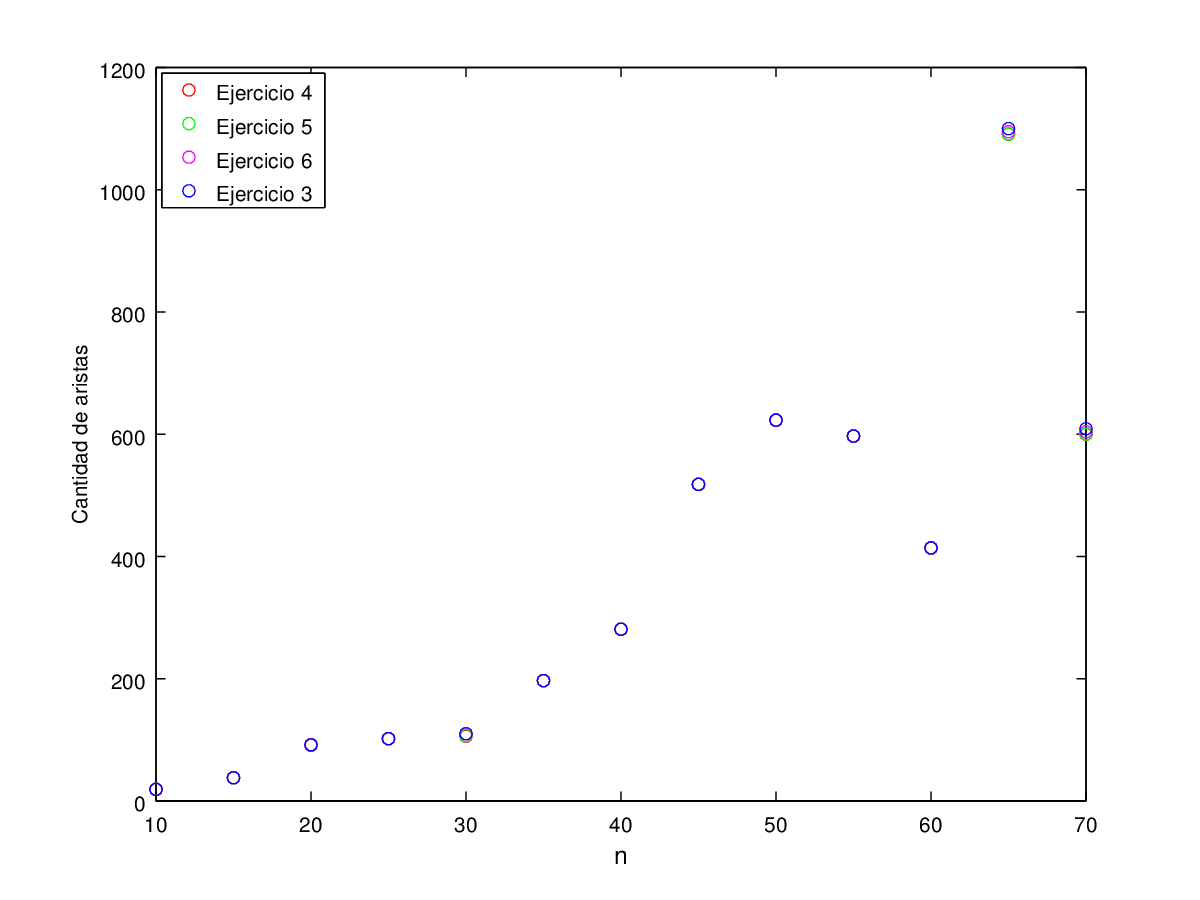
\includegraphics[height=10cm]{graficos/ejercicio7-exp4-comb1.png}
       \caption{Experimento 4- cografo y completo}
	\end{figure}
    
      \begin{figure}[H]
      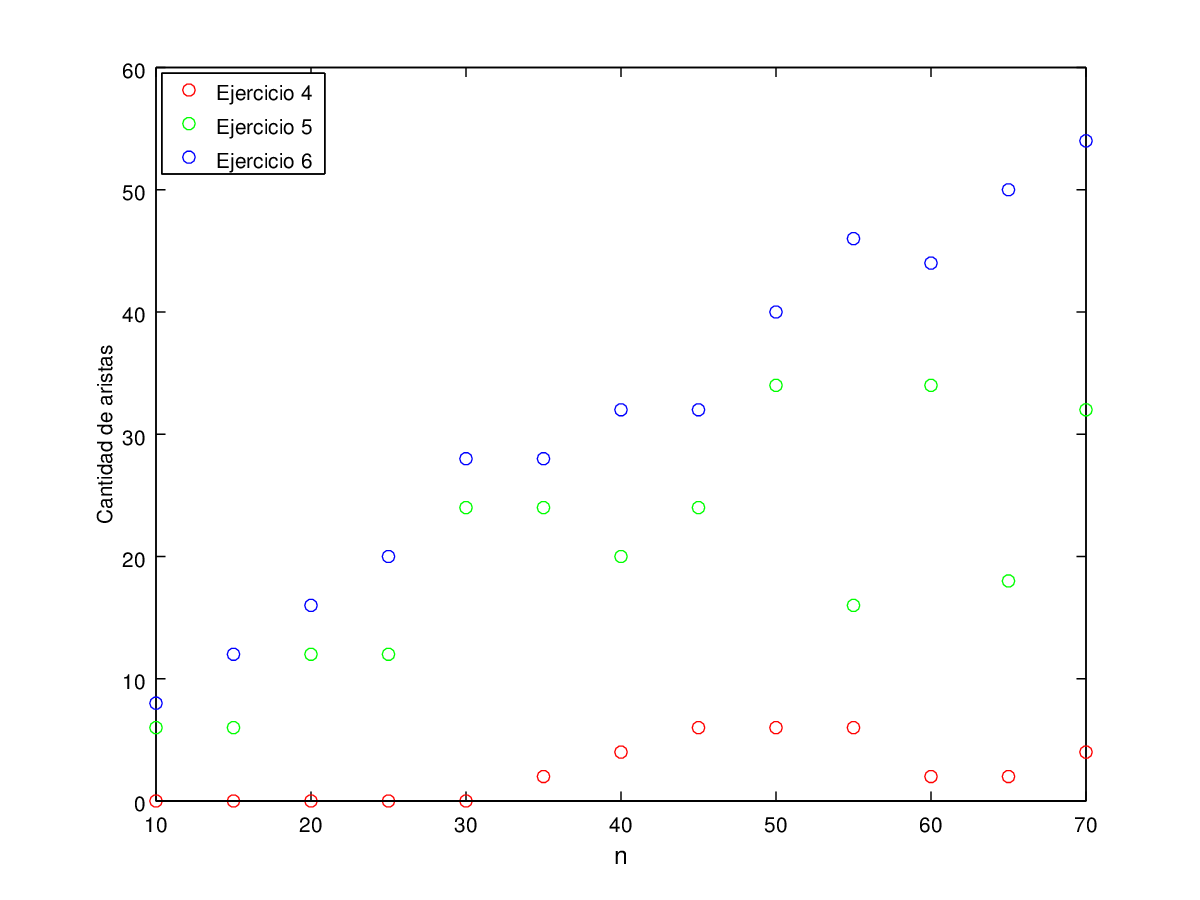
\includegraphics[height=10cm]{graficos/ejercicio7-exp4-comb2.png}
       \caption{Experimento 4- $C_n$ y bipartito completo}
	\end{figure}
    
      \begin{figure}[H]
      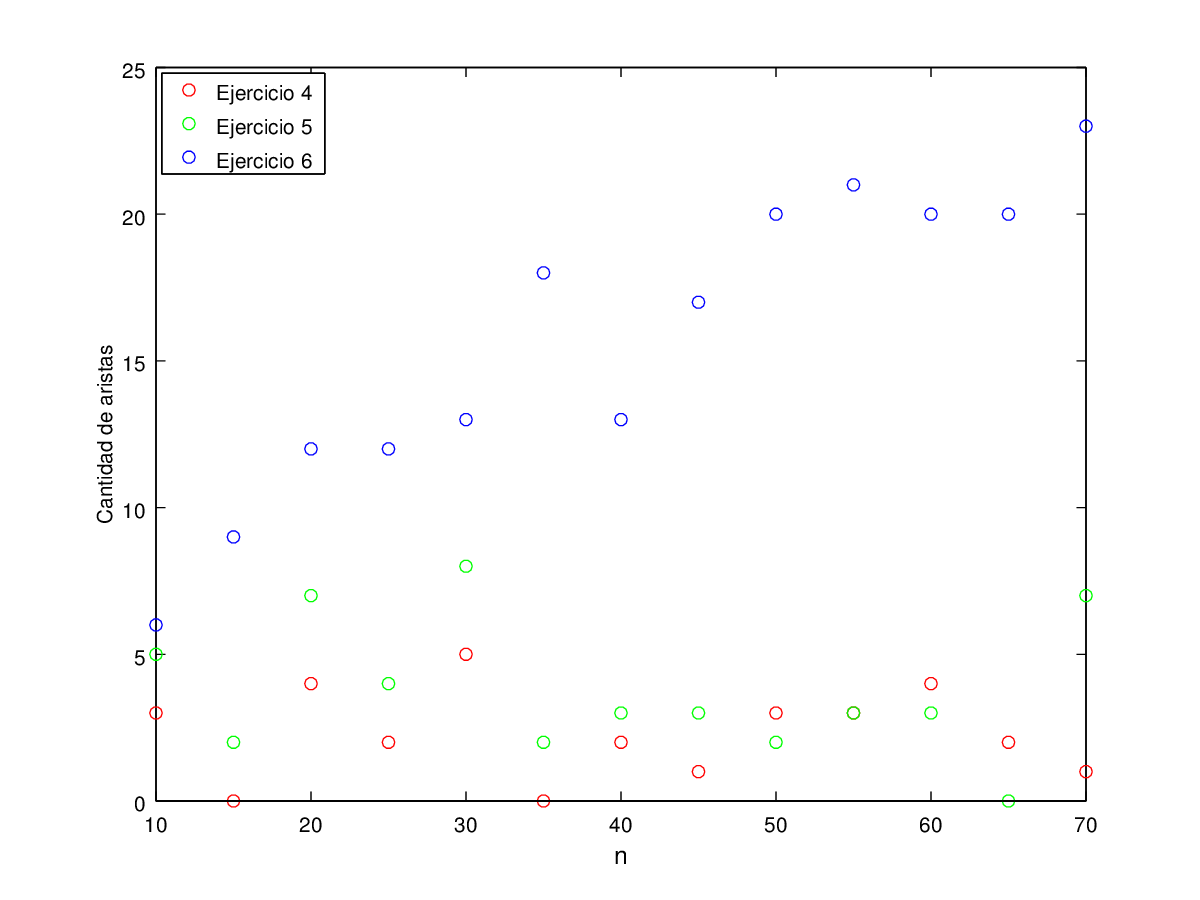
\includegraphics[height=10cm]{graficos/ejercicio7-exp4-comb3.png}
       \caption{Experimento 4- árbol y $C_n$}
	\end{figure}
    
    
    
\subsubsection*{Conclusiones}\;
En estos 3 grafos se observan diferentes comportamientos.\\
\begin{itemize}
\item En el primero que compara la cantidad de aristas de las solución de entre un cografo y un completo (las hip del Ej. 3), observamos que todos los algoritmos heurísticos son muy similares (cuando no iguales) al optimo, esto se lo atribuimos a que la heurística golosa es extremadamente eficaz en este caso particular, ya que el ordenar por grados y agarrar los vértices de mayor grado parece funcionar muy bien. Las otras 2 heurísticas parten del goloso y por lo tanto parten con una base muy solida para encontrar una mejor solución (El goloso en el peor caso mostró un margen de error respecto al optimo menor al 2\% para los casos probados).\\
En base a esto concluimos que si bien el mejor algoritmo para resolver este problema es exacto, pues encuentra la mejor solución y es el único que puede dar garantías, para entradas similares, por ejemplo, entre un cografo y un grafo casi completo o entre un grafo similar a un cografo y uno similar a un completo, incluso quizás entre uno relativamente con bastante aristas y uno casi completo, tendrá soluciones de una calidad aceptable, en un tiempo razonable, ya que podrá usar la metaheurística Tabú, o la búsqueda local si se quiere acortar los tiempos o incluso la heurística golosa que tiene un desempeño considerablemente mejor en tiempo de ejecución y aun así podría uno esperar en estos casos una solución de alta calidad.\\
\item En el segundo gráfico que se comparan los algoritmos heurísticos, ahora si sin un algoritmo exacto para comparar , ente un $C_n1$ y un $K_{n_2}$, se observa en este caso que la heurística golosa, contrariamente al caso anterior no es muy buena,en ningún caso encuentra mas de 10 aristas mientras que las otras heurísticas superan ampliamente ese numero (excepto en el caso n=10).\\
Se ve por otro lado que si bien la heurística goloso es mala, tanto la heurística de búsqueda local, como la metaheurística parecen ser considerablemente mejores y que la cantidad de aristas que encuentran en la solución es lineal en la cantidad de nodos(lo cual es bastante bueno, considerando que $C_n$ tiene $n$ aristas).\\
Considerando que si bien es notablemente mejor usar el algoritmo de heurística Tabú en esta situación si se quiere maximizar la cantidad de aristas, la decisión de utilizar este o el algoritmo de búsqueda local debe ser tomada considerando que el algoritmo de búsqueda local se ejecuta de manera mucho mas rápida.\\
Concluimos entonces que los mejores algoritmos para este tipo de instancias en particular, serán el de heurística Tabú, si lo que se quiere es encontrar la mejor solución posible o el de búsqueda local si lo que se quiere es una solución aceptable, pero que se ejecute en un periodo de tiempo mas corto.\\
No recomendamos para este tipo de instancia utilizar la heurística golosa ya que, si bien sera mas veloz en el tiempo de computo, la calidad de la solución es decir la cantidad de aristas, sera mucho mas baja.
\item En este último gráfico, se aprecia la experimentación rápidan de los algoritmos heurísticos ya mencionados entre un árbol y un $C_n$, tanto la heurística golosa como la heurística de búsqueda local, no parecen ser efectivas para encontrar una solución de calidad (al menos no de la calidad que encuentra la heurística Tabú).\\
En contraposición , la meta-heurística Tabú, si parece dar soluciones de calidad, ya que como notamos antes, la cantidad de aristas de la solución tiene un crecimiento lineal, lo que es mucho decir considerando que $C_n$ tiene $n$ aristas y un árbol de $n_2$ nodos tiene $n_2-1$ aristas.\\
Por lo tanto concluimos que si se quisiese resolver el problema con instancias de este tipo o similares, el algoritmo heurístico de Tabú es el mas recomendado a pesar de ser mas lento en cuanto a su tiempo de computo.\\
De necesitarse un algoritmo de resolución mas rápida, sugeriríamos plantear otra heurística golosa que se adapte mejor a la situación.\\
En caso que el tiempo se un factor decisivo y estemos obligados a elegir una de las 2 heurísticas mas veloces ya implementadas, la heurística golosa seria la indicada ya que la calidad de las soluciones sera baja en ambos casos pero el tiempo de computo sera sustancialmente mas corto.

\end{itemize}
Como conclusión general de  estas 3 instancias distintas del problema, observamos que cada una de las 3 heurísticas puede ser mas conveniente en distintos escenarios, esta en el análisis, la experimentación y el conocimiento del contexto de uso así como de las limitaciones y requerimientos temporales el cual es la mejor opción a elegir.